% 图 83.1 —— 由 `checks/emit_hand.py` 自动拼出（probe 精测 + prims2 图元分解）
%%
% ⚠ 这是**稿子不是成品**：跑 `checks/checkhand.py 83.1` 看指标 + 看叠合图。
%%
%% ⚠ 待核：
%   · 本图 probe 报出阴影族 1 个 —— **本脚本不生成阴影**（要照原书手写）；prims2 的 strokes 里可能含阴影线，核对时留意别画重
%   · 可疑字形 1 项（空心圈 ⊙ 常被认成字母 o）—— 见文件末
%%
\documentclass[12pt]{standalone}
\usepackage{fontspec}
\setsansfont{Arial}
\newfontfamily\mfallback{DejaVu Sans}
\usepackage{tikz}
\begin{document}
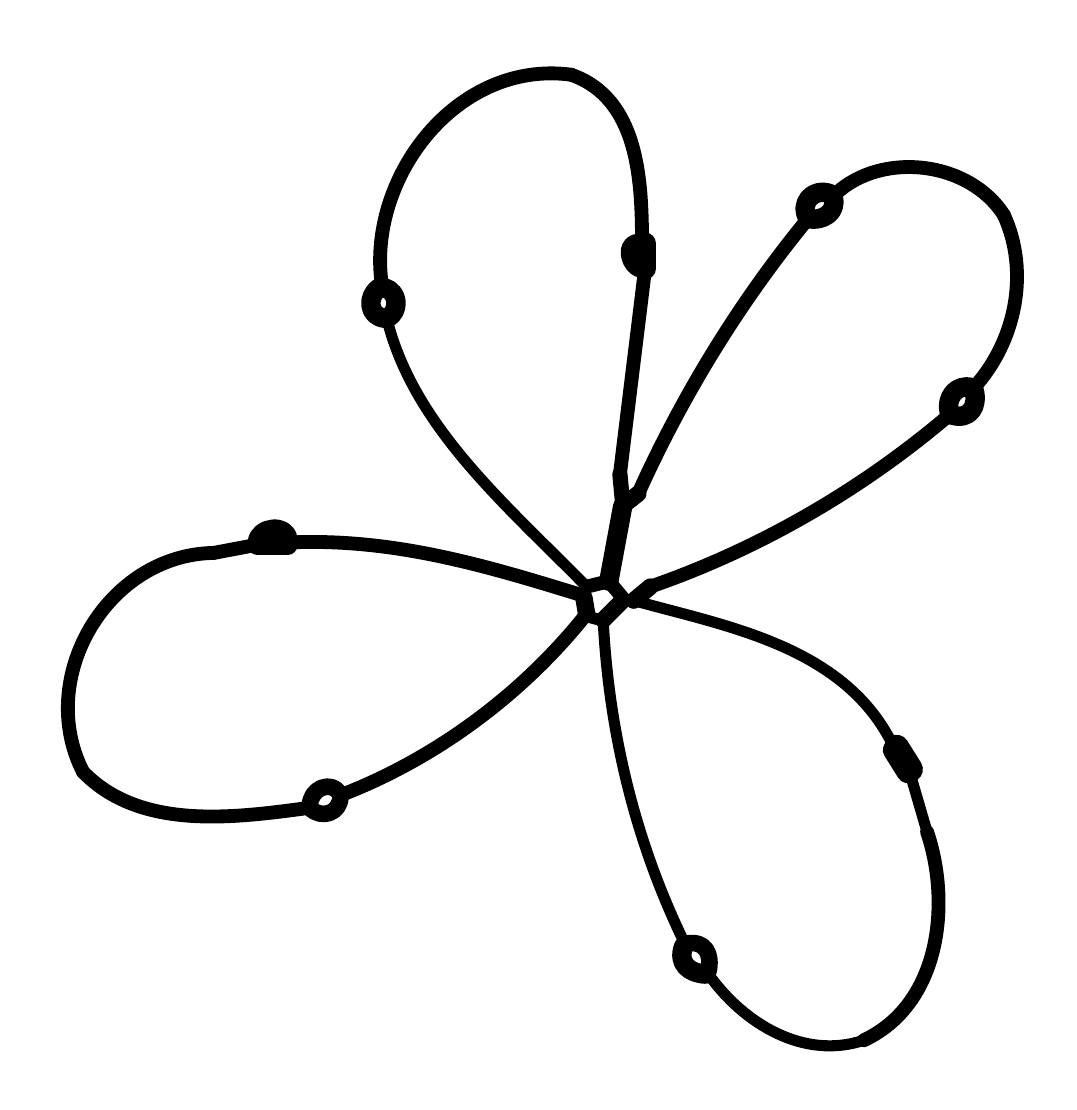
\begin{tikzpicture}[x=1pt, y=-1pt, line width=7.0pt, line cap=round, line join=round]

  %% ════ 直线段（prims2 的 strokes）════
  \draw[line width=7.0pt] (210.0,200.0) -- (215.0,173.0);
  \draw[line width=5.0pt] (210.0,200.0) -- (202.0,202.0);
  \draw[line width=5.0pt] (210.0,200.0) -- (215.0,206.0);
  \draw[line width=7.0pt] (94.0,187.0) -- (83.0,187.0);
  \draw[line width=6.0pt] (215.0,207.0) -- (208.0,214.0);
  \draw[line width=5.5pt] (215.0,172.0) -- (214.0,161.4);
  \draw[line width=5.0pt] (214.0,161.4) -- (223.0,88.0);
  \draw[line width=6.3pt] (202.0,212.0) -- (201.0,206.0);
  \draw[line width=8.0pt] (223.0,87.0) -- (223.0,78.0);
  \draw[line width=5.0pt] (82.0,187.0) -- (67.2,189.8);
  \draw[line width=9.0pt] (319.0,268.0) -- (314.0,260.0);
  \draw[line width=8.0pt] (318.0,269.0) -- (313.0,261.0);
  \draw[line width=4.0pt] (319.0,270.0) -- (325.0,290.6);
  \draw[line width=4.3pt] (203.0,213.0) -- (207.0,214.0);
  \draw[line width=6.0pt] (216.0,172.0) -- (220.6,168.4);
  \draw[line width=3.0pt] (216.0,207.0) -- (219.0,207.0);
  \draw[line width=6.0pt] (219.0,207.0) -- (225.0,202.0);

  %% ════ 曲线（prims2 的 curves —— 三段式，坐标同为 (y,x)）════
  \draw[line width=5.0pt] (95.0,186.0) .. controls (132.5,184.4) and (166.3,194.6) .. (200.0,205.0);
  \draw[line width=4.0pt] (313.0,260.0) .. controls (295.7,223.5) and (252.7,216.4) .. (219.0,207.0);
  \draw[line width=7.0pt] (245.0,342.0) .. controls (239.2,341.7) and (234.7,338.3) .. (237.0,332.0);
  \draw[line width=7.0pt] (341.0,130.0) .. controls (335.4,128.7) and (331.7,133.8) .. (333.0,139.0);
  \draw[line width=7.0pt] (342.0,131.0) .. controls (343.5,136.8) and (340.5,141.9) .. (334.0,140.0);
  \draw[line width=4.0pt] (237.0,330.0) .. controls (219.8,294.4) and (210.2,255.7) .. (208.0,215.0);
  \draw[line width=6.0pt] (102.0,282.0) .. controls (106.2,286.2) and (112.9,283.8) .. (113.0,278.0);
  \draw[line width=5.0pt] (201.0,213.0) .. controls (178.1,241.5) and (146.9,264.2) .. (114.0,277.0);
  \draw[line width=6.0pt] (246.0,341.0) .. controls (247.4,334.8) and (244.9,329.6) .. (238.0,331.0);
  \draw[line width=5.0pt] (67.2,189.8) .. controls (28.9,190.4) and (2.6,234.8) .. (20.0,268.9);
  \draw[line width=5.0pt] (20.0,268.9) .. controls (40.5,290.1) and (74.2,285.6) .. (101.0,282.0);
  \draw[line width=7.0pt] (290.0,60.0) .. controls (283.8,57.7) and (278.6,63.4) .. (282.0,69.0);
  \draw[line width=7.0pt] (127.0,94.0) .. controls (122.4,97.2) and (123.1,104.4) .. (129.0,105.0);
  \draw[line width=7.0pt] (130.0,105.0) .. controls (134.5,102.5) and (134.1,95.4) .. (129.0,94.0);
  \draw[line width=5.0pt] (128.0,93.0) .. controls (122.3,54.9) and (154.7,11.4) .. (196.4,17.0);
  \draw[line width=5.0pt] (196.4,17.0) .. controls (220.6,25.5) and (221.9,54.7) .. (222.0,77.0);
  \draw[line width=5.0pt] (325.0,290.6) .. controls (333.8,316.7) and (329.7,353.0) .. (302.1,365.9);
  \draw[line width=4.0pt] (302.1,365.9) .. controls (280.6,373.1) and (258.7,360.0) .. (246.0,342.0);
  \draw[line width=7.0pt] (222.0,87.0) .. controls (217.7,86.5) and (215.6,77.7) .. (221.0,78.0);
  \draw[line width=6.0pt] (102.0,281.0) .. controls (102.0,275.3) and (109.3,271.3) .. (113.0,277.0);
  \draw[line width=5.0pt] (342.0,130.0) .. controls (357.1,113.3) and (362.1,88.3) .. (352.8,67.8);
  \draw[line width=5.0pt] (352.8,67.8) .. controls (340.3,48.1) and (308.7,44.5) .. (292.0,60.0);
  \draw[line width=7.0pt] (291.0,61.0) .. controls (292.8,66.8) and (287.1,70.1) .. (282.0,69.0);
  \draw[line width=4.0pt] (201.0,201.0) .. controls (172.8,172.3) and (139.8,144.4) .. (130.0,106.0);
  \draw[line width=5.0pt] (220.6,168.4) .. controls (236.3,133.5) and (256.9,99.5) .. (282.0,69.0);
  \draw[line width=7.0pt] (94.0,185.0) .. controls (93.7,179.2) and (83.3,180.4) .. (83.0,186.0);
  \draw[line width=5.0pt] (225.0,202.0) .. controls (264.0,188.5) and (300.9,167.3) .. (333.0,140.0);

  %% ════ 标签（probe 直接给的 \node 行）════
  %% ⚠ 全部补了 fill=white：文字在最上层，否则与曲线交叉干扰

  % 钉死画布：否则超出的图元/控制点会把页面撑大，1:1 回比就失准
  \pgfresetboundingbox
  \path[use as bounding box] (0,0) rectangle (369,381);
\end{tikzpicture}
\end{document}

% ⚠ 待核清单（probe 拿不准，人眼过一遍）：
%   · 未识别/跳过：⑤ 跳过/未识别的字形
